\chapter{Introduzione}
\section{Differenza Fra Artificial Intelligence e Generative Artificial Intelligence}
La prima domanda, che ci sorge in mente quando leggiamo il nome del corso è:
\begin{center}
    \textbf{Qual è la differenza fra "Artificial Intelligence" (AI) e "Generative Artificial Intelligence" (GAI)}
\end{center}
Cerco di spiegarmi nel modo piu chiaro possibile:
\begin{itemize}
    \item \textbf{AI} : L'AI analizza dati esistenti attraverso compiti supervisionati (classificazione, regressione), 
    non supervisionati (clustering, riduzione di dimensionalità) o self-supervised 
    (es. modellazione del linguaggio), a seconda dell'approccio.
    \begin{example}{Esempio di utilizzo di AI}
        Per esempio immagina di avere tante foto di animali,l'AI analizza le immagini e classifica ciascuna immagine, quindi l'output è legato
        ai dati che abbiamo fornito
    \end{example}
    \begin{observation}{Dati supervisionati,non supervisionati e self-supervised}
        \begin{itemize}
            \item \textbf{Dati Supervisionati (Supervised learning)} : Ho un input + la risposta corretta (label)
            \item \textbf{Dati non Supervisionati (Unsupervised learning)} : Ho solamente gli input, senza una risposta corretta.
            \item \textbf{Supervisione creata dai dati (Self-supervised learning)} : Anche qui non ho label fornite da esseri umani, 
            ma costruisci automaticamente un compito supervisionato usando i dati stessi. \textbf{Cioè nascondo una parte di Informazione
            e chiedo al modello di prevederla}
            Per esempio prendiamo una frase:
            \begin{center}
                Il gatto mangia il pesce
            \end{center}
            Nascondiamo una parola
            \begin{center}
                Il gatto mangia [MASK]
            \end{center}
            e chiediamo al modello
            \begin{center}
                Qual è la parola mancante?
            \end{center}
            il target è : "pesce".

            \textbf{La cosa importante è che "pesce" non era una label fornita dall'esterno, ma stava nei dati originali e costruisco quindi un compito
            supervisionato usando i dati stessi}
        \end{itemize}
    \end{observation}
    \newpage
    \item \textbf{GAI} : Categoria di AI che genera \textbf{nuovi contenuti}, questo include
    \begin{itemize}
        \item \textbf{Generare testo}
        \item \textbf{Generare immagini}
        \item \textbf{Generare video}
        \item \dots
    \end{itemize}
    Il modello ha imparato pattern dai dati di addestramento e li usa per produrre nuovi output.
\end{itemize}
\section{Come funziona Generative AI (In generale)}
L'AI generativa è tipicamente basata sul deep learning, specialmente parliamo di modelli allenati su grandi dataset, usando neural network architectures
\begin{itemize}
    \item Transformers (GPT,BERT,\dots)
    \item GANs (Generative Adversarial Network) - popolari per le immagini
    \item VAEs (Variational Autoencoders)
\end{itemize}
\begin{figure}[h]
    \centering
    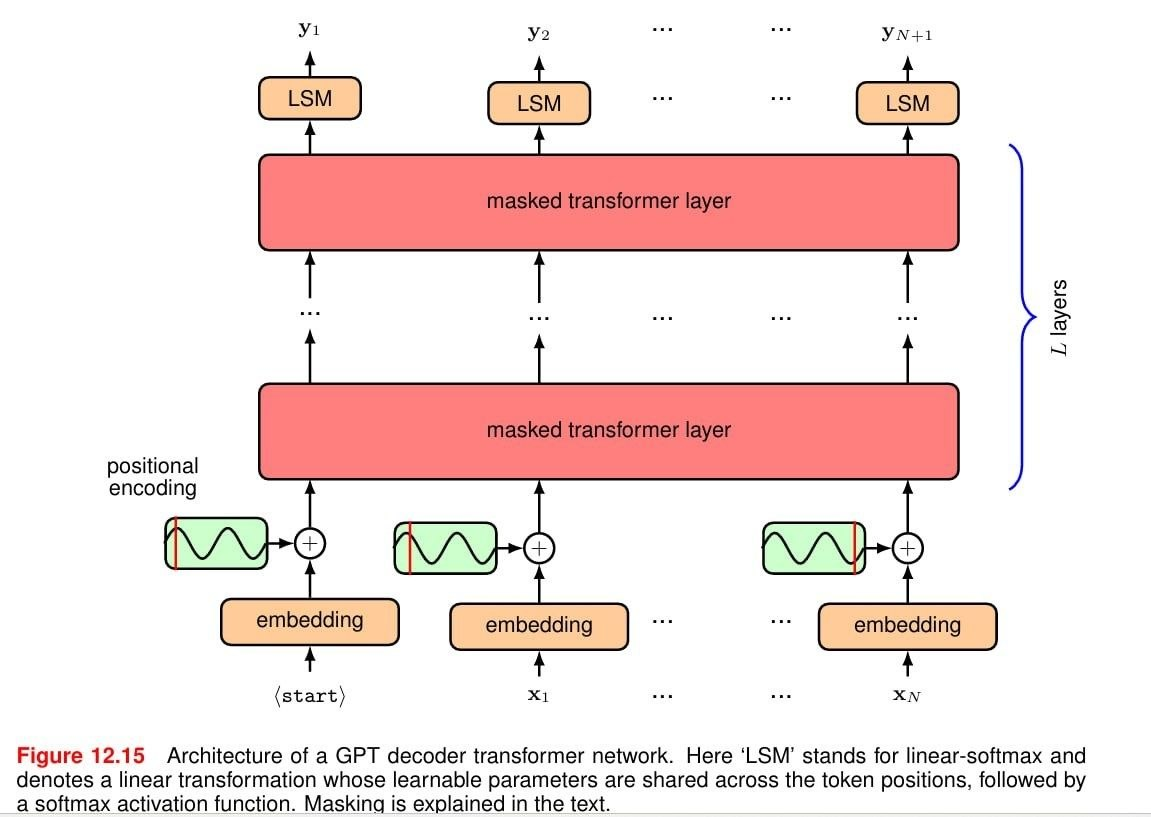
\includegraphics[width=0.8\textwidth]{_files/_images/GPT.png}
    \caption{Archittetura di GPT}
    \label{fig:GPT}
\end{figure}
Quindi in sostanza l'IA generativa,genera nuovi contenuti, come testo,immagini e audio, questo lo fa tramite modelli allenati su grandi dataset, modelli del tipo reti neurali.
Un esempio di modello che genera testo è \textbf{Generative Language Models}
\newpage
\section{Generative AI : Applicazioni e Limitazioni}
L'AI generativa trova applicazioni in:
\begin{itemize}
    \item \textbf{Creative Work}
    \item \textbf{Content Generation}
    \item \textbf{Software Development}
    \item \textbf{Education and tutoring}
    \item \textbf{Ricerche Mediche}
    \item \textbf{Generazione di testo}
\end{itemize}
ma ci sono da considerare anche i limiti che questa ha ora:
\begin{itemize}
    \item \textbf{Allucinazioni} : Le allucinazioni dell'AI sono casi in cui un modello di intelligenza artificiale genera informazioni 
    false o non supportate dai dati, presentandole però in modo plausibile e sicuro.
    Un'allucinazione non significa necessariamente che l'AI "sa che è falso e mente", la differenza è:
    \begin{itemize}
        \item \textbf{Menzogna} : Si conosce la verità,ma dico deliberatamente qualcosa di falso
        \item \textbf{Allucinazione} : L'IA genera una risposta pI Language Models sono un'applicazione della Generative AI nel dominio del testo, ovvero modelli specializzati nella generazione di linguaggio naturalelausibile,ma quella è falsa.
    \end{itemize}
    \item \textbf{DeepFakes} : l'AI genera/manipola immagini, video o audio per rappresentare una persona o un evento in modo falso.
\end{itemize}
